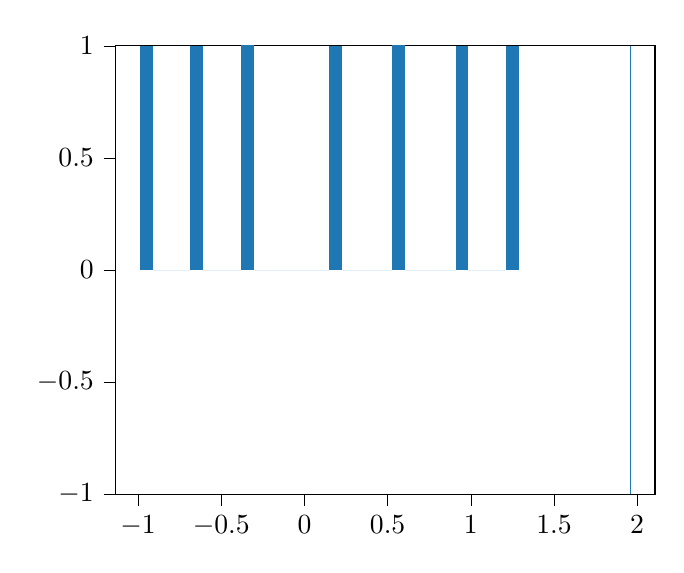
\begin{tikzpicture}

\definecolor{darkgray176}{RGB}{176,176,176}
\definecolor{steelblue31119180}{RGB}{31,119,180}

\begin{axis}[
tick align=outside,
tick pos=left,
x grid style={darkgray176},
xmin=-1.1365774, xmax=2.1074561,
xtick style={color=black},
y grid style={darkgray176},
ymin=-1, ymax=1,
ytick style={color=black}
]
\draw[draw=none,fill=steelblue31119180] (axis cs:-0.98912135,0) rectangle (axis cs:-0.9132198,1);
\draw[draw=none,fill=steelblue31119180] (axis cs:-0.9132198,0) rectangle (axis cs:-0.83731824,0);
\draw[draw=none,fill=steelblue31119180] (axis cs:-0.83731824,0) rectangle (axis cs:-0.76141669,0);
\draw[draw=none,fill=steelblue31119180] (axis cs:-0.76141669,0) rectangle (axis cs:-0.68551514,0);
\draw[draw=none,fill=steelblue31119180] (axis cs:-0.68551514,0) rectangle (axis cs:-0.60961358,1);
\draw[draw=none,fill=steelblue31119180] (axis cs:-0.60961358,0) rectangle (axis cs:-0.53371203,0);
\draw[draw=none,fill=steelblue31119180] (axis cs:-0.53371203,0) rectangle (axis cs:-0.45781047,0);
\draw[draw=none,fill=steelblue31119180] (axis cs:-0.45781047,0) rectangle (axis cs:-0.38190892,0);
\draw[draw=none,fill=steelblue31119180] (axis cs:-0.38190892,0) rectangle (axis cs:-0.30600737,3);
\draw[draw=none,fill=steelblue31119180] (axis cs:-0.30600737,0) rectangle (axis cs:-0.23010581,0);
\draw[draw=none,fill=steelblue31119180] (axis cs:-0.23010581,0) rectangle (axis cs:-0.15420426,0);
\draw[draw=none,fill=steelblue31119180] (axis cs:-0.15420426,0) rectangle (axis cs:-0.078302706,0);
\draw[draw=none,fill=steelblue31119180] (axis cs:-0.078302706,0) rectangle (axis cs:-0.002401152,0);
\draw[draw=none,fill=steelblue31119180] (axis cs:-0.002401152,0) rectangle (axis cs:0.073500402,0);
\draw[draw=none,fill=steelblue31119180] (axis cs:0.073500402,0) rectangle (axis cs:0.14940196,0);
\draw[draw=none,fill=steelblue31119180] (axis cs:0.14940196,0) rectangle (axis cs:0.22530351,1);
\draw[draw=none,fill=steelblue31119180] (axis cs:0.22530351,0) rectangle (axis cs:0.30120506,0);
\draw[draw=none,fill=steelblue31119180] (axis cs:0.30120506,0) rectangle (axis cs:0.37710662,0);
\draw[draw=none,fill=steelblue31119180] (axis cs:0.37710662,0) rectangle (axis cs:0.45300817,0);
\draw[draw=none,fill=steelblue31119180] (axis cs:0.45300817,0) rectangle (axis cs:0.52890972,0);
\draw[draw=none,fill=steelblue31119180] (axis cs:0.52890972,0) rectangle (axis cs:0.60481128,2);
\draw[draw=none,fill=steelblue31119180] (axis cs:0.60481128,0) rectangle (axis cs:0.68071283,0);
\draw[draw=none,fill=steelblue31119180] (axis cs:0.68071283,0) rectangle (axis cs:0.75661439,0);
\draw[draw=none,fill=steelblue31119180] (axis cs:0.75661439,0) rectangle (axis cs:0.83251594,0);
\draw[draw=none,fill=steelblue31119180] (axis cs:0.83251594,0) rectangle (axis cs:0.90841749,0);
\draw[draw=none,fill=steelblue31119180] (axis cs:0.90841749,0) rectangle (axis cs:0.98431905,1);
\draw[draw=none,fill=steelblue31119180] (axis cs:0.98431905,0) rectangle (axis cs:1.0602206,0);
\draw[draw=none,fill=steelblue31119180] (axis cs:1.0602206,0) rectangle (axis cs:1.1361222,0);
\draw[draw=none,fill=steelblue31119180] (axis cs:1.1361222,0) rectangle (axis cs:1.2120237,0);
\draw[draw=none,fill=steelblue31119180] (axis cs:1.2120237,0) rectangle (axis cs:1.2879253,1);
\addplot [semithick, steelblue31119180]
table {%
1.96 -1
1.96 1
};
\end{axis}

\end{tikzpicture}
